\documentclass[usenames,dvipsnames]{beamer}
  \usepackage{times}
  \usepackage{xcolor}
  \usepackage{tcolorbox}
  \usepackage{amsmath,amsthm, amssymb}
  \boldmath
  \usetheme{RedLion}
  \usepackage[orientation=portrait,size=a1,scale=1.4]{beamerposter}
  
  \title[https://arxiv.org/abs/2307.00177]{Homological Quillen's fiber lemma for persistence posets}
  \author[viviag@yandex.ru, viviag.io]{Vitalii Guzeev}
  \institute[HSE]{HSE faculty of mathematics}
  \date{24/07/2023}

  \logo{
\includegraphics[scale=0.05]{arxiv-link.eps}}

  %%%%%%%%%%%%%%%%%%%%%%%%%%%%%%%%%%%%%%%%%%%%%%%%%%%%%%%%%%%%%%%%%%%%%%%%%%%%%%%%%5
  \begin{document}
  \begin{frame}{}
    \begin{block}{\large Motivation}
      \centering
      {\normalsize Complexity of persistent homology computation is a concern.\par
      It would be nice to have an algorithm to reproducibly reduce a persistence complex (as experimental data) to a smaller one.}\par
    \end{block}
    \vspace{0.5cm}
    \begin{tcolorbox}[ size=tight,oversize,sharp corners
                     , colback=taspruce,colframe=ta2aluminium,left=56pt,right=90pt,bottom=20pt
                     ]
    \begin{minipage}{0.97\paperwidth}
    \begin{columns}[t]
      \begin{column}{.48\linewidth}
        \begin{block}{Quillen's fiber lemma}
          Let $X, Y \in Pos$ be finite, $f : X \to Y$ be a morphism.\\
    If $\forall y \in Y\;B(f^{-1}(Y_{\leqslant y}))$ is contractible, then $Bf$ is a homotopy equivalence between $BX$ and $BY$.
        \end{block}
      \end{column}
      \begin{column}{.51\linewidth}
        \begin{block}{Homological Quillen's fiber lemma}
          Let $X, Y \in Pos$ be finite, $f : X \to Y$ be a morphism, $R$ be a PID.\\
    If $\forall y \in Y\;H_i(B(f^{-1}(Y_{\leqslant y})),R) = 0$ for any $i$, then $Bf$ induces isomorphisms of all homology modules with coefficients in $R$ on $BX$ and $BY$.
        \end{block}
      \end{column}
    \end{columns}
    \begin{block}{\large Jonathan Barmak's proof of homological Quillen's fiber lemma}
      \begin{minipage}{0.97\linewidth}
      \begin{columns}[t]
      \begin{column}{.27\linewidth}
        \begin{block}{Covering}
          Let $x$ be an element in a poset $X$.\par
          Then $BX = B(X \setminus \{x\}) \cup \left|\operatorname{st}(\mathcal{N}(x))\right|$
        \end{block}
      \end{column}
      \begin{column}{.30\linewidth}
        \begin{block}{Mapping cylinder}
          The set $M(f) = X \coprod Y$ with the order $R = R_X \cup R_Y \cup \{(x,f(x))\;|\;\forall x \in X\}$.
        \end{block}
      \end{column}
      \begin{column}{.42\linewidth}
        \begin{block}{Major lemma}
          Under conditions of the theorem, the inclusion $B(X \setminus \{x\}) \to BX$ induces isomorphisms of all homology modules.
        \end{block}
      \end{column}
    \end{columns}
    \begin{block}{Proof scheme}
      For the lemma: Kunneth formula for a join and Mayer-Vietoris l.e.s.\par
      For the theorem: $B(M(f))$ retracts to $BY$. Extend order on $Y$ to linear and iterate the lemma, adding elements of $Y$ to $X$ one by one.
    \end{block}
      \end{minipage}
    \end{block}
    \end{minipage}
    \end{tcolorbox}
    \begin{columns}[t]
        \begin{column}{.22\linewidth}
            \begin{block}{Persistence objects}
              $Fun_{Cat}(I, \mathcal{C})$ for posetal category $I$ and given $\mathcal{C}$.\par
              {\small Many constructions work index-wise, e.g. mapping cylinder.}\par
            \end{block}
            \begin{block}{Persistence subposet}
              $X \subset Y$ if for each $i \in I$ $X_i$ embeds to $Y_i$ and everything commutes.
            \end{block}
            \begin{block}{Element of a persistence poset}
              $x \in X$ if $x \subset Y$ and for each $i$ $\#x_i \leq 1$.\par
              Equivalently, it is an element $x_i \in X_i$ for some $i$ and its images under structure maps.
            \end{block}
            \begin{block}{Persistence covering of BX}
              $X = \bigcup X_i$ and $BX \sim \bigcup BX_i$\par
              Barmak's covering extends to a persistence one.
            \end{block}
        \end{column}
      \begin{column}{0.0001\linewidth}
          \begin{center}
          \rule{2pt}{0.4\textheight}
          \end{center}
      \end{column}
      \begin{column}{.38\linewidth}
        \begin{block}{Object of finite type}
          Persistence poset of finite type --- finite sequence of finite posets; module --- of finitely generated modules.
        \end{block}
        \begin{block}{\large MAIN RESULT}
          Assume $X, Y$ are persistence posets of finite type indexed by a totally ordered good monoid $I$, $f : X \to Y$ is an order-preserving map. Let $m$ be the number of elements of $Y$ and $R$ is a PID.\\

          Then if $\forall y \in Y\;B(f^{-1}(Y_{\leqslant y}))$ is $\varepsilon$-acyclic over $R$, $BX$ and $BY$ are $4m\varepsilon$-interleaved over $R$.
        \end{block}
        \begin{block}{Persistent order extension principle}
          An order on elements is defined by a first non-empty component. Assume $I$ is totally ordered. Then elements are ordered by pair (birth index $i$, order of $x_i \in X_i$).\par
          \vspace{0.1cm}
          Series $X'_i$ of extensions of $X_i$ is an extension of a persistence poset $X$ if structure maps of $X$ are well-defined on $X'$. An extension that is a series of linear extensions is called a linear extension.\par
          \vspace{0.1cm}
          Consider the set of extensions of $X$ ordered by inclusion and apply Zorn's lemma.\par
          No need in Zorn's lemma for a finite-type case.
        \end{block}
      \end{column}
      \begin{column}{0.0001\linewidth}
          \begin{center}
          \rule{2pt}{0.4\textheight}
          \end{center}
      \end{column}
      \begin{column}{.38\linewidth}
        \begin{block}{Interleaving distances}
          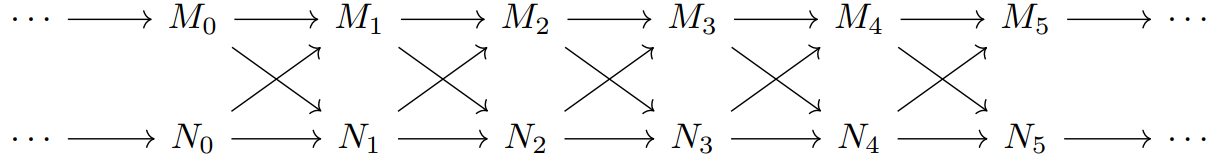
\includegraphics[scale=0.45]{wiki_interleaving.png} (wiki)\par
          $d(X,Y) = min\{\varepsilon \in I\;|\;X \stackrel{\varepsilon}{\sim} Y\}$
        \end{block}
        \begin{block}{Correspondence theorem (Corbet, Kerber 2018)}
          Let $R$ be a ring with unity and $G$ be a good monoid (Definition 2.16, follow the QR code). Then the category of finitely presented graded $R[G]$-modules is isomorphic to the category of $G$-indexed persistence modules over $R$ of finitely presented type.
        \end{block}
        \begin{block}{Stability in $G$-indexed persistence modules}
          All results rely on stability in short exact sequences (Lemma 2.24).\par
          \begin{itemize}
          \item $d(A, 0) \leq \varepsilon; d(B, 0) \leq \varepsilon$ imply $d(A \oplus B, 0) \leq \varepsilon; d(A \otimes B, 0) \leq \varepsilon$
          \item Let $P$ be a chain complex with $d(P_i,0) \leq \varepsilon$. Then $d(H_i(P),0) \leq \varepsilon$ ($P$ is $\varepsilon$-acyclic).
          \item $d(A,0) \leq \varepsilon$ or $d(B,0) \leq \varepsilon$ imply $d(Tor_i(A,B),0) \leq \varepsilon$.
          \item Let $A \to B \to C \to D$ be exact. Then $d(A,0) \leq \varepsilon$ and $d(D,0) \leq \varepsilon$ imply $B \stackrel{4\varepsilon}{\sim} C$.
          \end{itemize}
        \end{block}
      \end{column}
    \end{columns}
    \begin{columns}[t]
      \begin{column}{.70\linewidth}
        \begin{block}{Major lemma}
          Let $BX_{< x}$ or $BX_{> x}$ be $\varepsilon$-acyclic. Then persistent homology of $B(X \setminus \{x\})$ and $B(X)$ are $4\varepsilon$-interleaved.
        \end{block}
      \end{column}
      \begin{column}{.13\linewidth}
        \begin{block}{Proof scheme}
          \centering
          Applies.
        \end{block}
      \end{column}
    \end{columns}
    \begin{block}{Further work}
      \centering
      An algorithm? Relax a PID requirement using the Kunneth s.s.? Something else?
    \end{block}
    \centering
    {\small The work was conducted in the Laboratory for Applied Geometry and Topology at HSE (preceding the ATA Lab) under the supervision of Anton Ayzenberg.}  
  \end{frame}
\end{document}

